\begin{figure}[tbp]
\centering
\begin{minipage}[c]{0.40\textwidth}
\centering
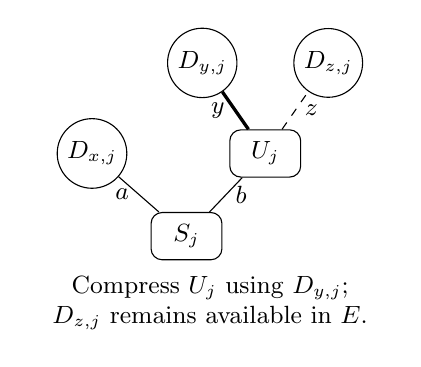
\begin{tikzpicture}[x=1cm,y=1cm,
 body/.style={draw,rounded corners,minimum width=9mm,minimum height=6mm},
 gropecap/.style={draw,circle,inner sep=2pt},
 every node/.style={font=\small}]
 \node[body] (s) at (0,0) {$S_j$};
 \node[gropecap] (a) at (-1.2,1.05) {$D_{x,j}$};
 \node[body] (u) at (1.0,1.05) {$U_j$};
 \node[gropecap] (y) at (0.2,2.2) {$D_{y,j}$};
 \node[gropecap] (z) at (1.8,2.2) {$D_{z,j}$};
 \draw (s)--node[left] {$a$}(a);
 \draw (s)--node[right] {$b$}(u);
 \draw[very thick] (u)--node[left] {$y$}(y);
 \draw[dashed] (u)--node[right] {$z$}(z);
 \node[align=center,text width=4.4cm] at (0.3,-0.85)
  {Compress \(U_j\) using \(D_{y,j}\);\\
   \(D_{z,j}\) remains available in \(E\).};
\end{tikzpicture}
\end{minipage}
\hfill
\begin{minipage}[c]{0.57\textwidth}
\centering
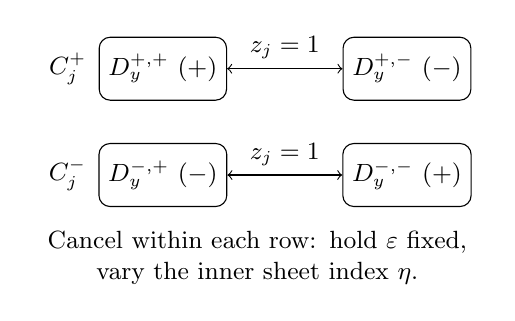
\begin{tikzpicture}[x=1cm,y=1cm,
 sheet/.style={draw,rounded corners,minimum width=1.45cm,minimum height=8mm},
 every node/.style={font=\small}]
 \node[sheet] (pp) at (0,1.1) {$D_y^{+,+}\ (+)$};
 \node[sheet] (pm) at (3.1,1.1) {$D_y^{+,-}\ (-)$};
 \node[sheet] (mp) at (0,-0.25) {$D_y^{-,+}\ (-)$};
 \node[sheet] (mm) at (3.1,-0.25) {$D_y^{-,-}\ (+)$};
 \draw[<->] (pp)--node[above] {$z_j=1$}(pm);
 \draw[<->] (mp)--node[above] {$z_j=1$}(mm);
 \node[anchor=east] at (-0.85,1.1) {$C_j^+$};
 \node[anchor=east] at (-0.85,-0.25) {$C_j^-$};
 \node[align=center,text width=5.6cm] at (1.2,-1.3)
  {Cancel within each row: hold \(\varepsilon\) fixed,\\
   vary the inner sheet index \(\eta\).};
\end{tikzpicture}
\end{minipage}
\caption{Combinatorial schematics, not projections of the four-dimensional
embedding. Left: the two-stage body and its one-sided upper contraction.
Right: the four occurrences of its surgery cap in the compressed rim
sphere; parentheses record their orientation coefficients
\(\varepsilon\eta\). The right panel suppresses the cap's subscript \(j\).
The labels \(z_j=1\) are equalities in \(\pi_1(E)\), proved using the upper
dual cap in \(E\).
No comparison between the two rows, which could involve a bottom
normal-circle meridian, is used.}
\label{fig:geometry-sheets}
\end{figure}
